\def\mytitle{\textbf{AVR-GCC ASSIGNMENT}}
\documentclass[10pt,a4paper]{article}
\usepackage[a4paper,outer=1.5cm,inner=1.5cm,top=1.75cm,bottom=1.5cm]{geometry}
\usepackage{graphicx}
\usepackage{tikz}
\usepackage{tabularx}
\usepackage{amsmath}
\title{\mytitle}
\author{Pavan Srinivas Marri\\marripavan65@gmail.com\\FWC22138 IITH - Future Wireless Communications}
\date{}
\begin{document}
\maketitle
\graphicspath{{./Documents}{./figs}}
\tableofcontents
\section{Problem}
(GATE2019-QP-EE)\\
Q.35 The output expression for the Karnaugh map shown below is
\begin{center}
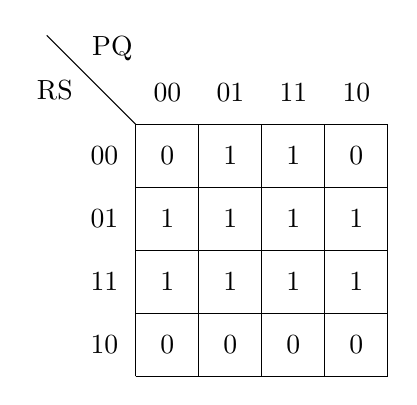
\begin{tikzpicture}[scale=0.8]
\draw (0,0) grid (4,4);
  \draw (0,4) -- node [pos=0.6,above right,anchor=south west] {PQ} node [pos=0.6,below left,anchor=north east] {RS} ++(135:2);  
  % Draw vertical lines
  \foreach \x in {0,1,2,3,4}
    \draw (\x,0) -- (\x,4);  
  % Draw horizontal lines
  \foreach \y in {0,1,2,3,4}
    \draw (0,\y) -- (4,\y);  
  % Draw cell labels
  %4th row
  \node at (0.5,0.5) {0};
  \node at (1.5,0.5) {0};
  \node at (2.5,0.5) {0};
  \node at (3.5,0.5) {0};
  %3rd row
  \node at (0.5,1.5) {1};
  \node at (1.5,1.5) {1};
  \node at (2.5,1.5) {1};
  \node at (3.5,1.5) {1};
  %2nd row
  \node at (0.5,2.5) {1};
  \node at (1.5,2.5) {1};
  \node at (2.5,2.5) {1};
  \node at (3.5,2.5) {1};
  %1st row
  \node at (0.5,3.5) {0};
  \node at (1.5,3.5) {1};
  \node at (2.5,3.5) {1};
  \node at (3.5,3.5) {0};
  % Draw index labels
  \foreach \x/\val in {0/00,1/01,2/11,3/10}
    \node at (\x+0.5,4.5) {\val};
   % Draw index labels    
  \foreach \y/\val in {3/00,2/01,1/11,0/10}
    \node at (-0.5,\y+0.5) {\val};
\end{tikzpicture}
\end{center}
\begin{enumerate}
	\item[(A)] $ Q\bar{R} + S $
	\item[(B)] $ QR + S $
	\item[(C)] $ Q\bar{R} + \bar{S} $
	\item[(D)] $ QR + \bar{S} $
\end{enumerate}
\section{Components}
\begin{table}[h]
	\centering
\begin{tabularx}{0.8\textwidth}{
		| >{\centering\arraybackslash}X
		| >{\centering\arraybackslash}X
		| >{\centering\arraybackslash}X |}
	\hline
	 \textbf{Components} & \textbf{Value} & \textbf{Quantity} \\
	\hline
	 Breadboard & - & 1 \\
	 \hline
	 Arduino & uno & 1 \\
	 \hline
	 Jumper wires &  & 4 \\
	 \hline
\end{tabularx}
\caption{Components}
\label{table:components}
\end{table}
\subsection{Arduino}
The Arduino Uno has some ground pins.analog input 
pins A0-A3 and digial pins D1-D13 that can be used
for both input as well as output. It also has two
powe pins that can generate 3.3V and 5V. In the
following exercise,we use digital pins,GND and 5V
\section{Implementation}
\subsection{Truth table}
\begin{table}[h]
	\centering
\begin{tabularx}{0.8\textwidth}{
		| >{\centering\arraybackslash}X
		| >{\centering\arraybackslash}X
		| >{\centering\arraybackslash}X | }
	\hline
	\textbf{Input A} & \textbf{Input B} & \textbf{Output}\\
	\hline
	0 & 0 & 1 \\
	\hline
	0 & 1 & 0 \\
	\hline
	1 & 0 & 0 \\
	\hline
	1 & 1 & 0 \\
	\hline
\end{tabularx}
	\caption{Truth Table}
	\label{table:truth_table}
\end{table}
\subsection{Boolean Equation}
\begin{align}
	F &= \bar{R}S\bar{P}(\bar{Q} + Q) + \bar{R}SP(\bar{Q} + Q) + \bar{R}\bar{S}Q(\bar{P} + P) + \bar{R}SQ(\bar{P} + P) + RS\bar{P}(\bar{Q} + Q) + RSP(\bar{Q} + Q) \\
	F &= \bar{R}S(\bar{P} + P) + \bar{R}Q(\bar{S} + S) + RS(\bar{P} + P) \\
	F &= S(\bar{R} + R) + \bar{R}Q \\
	F &= S + Q\bar{R} 
\end{align}
\section{Hardware}
\begin{enumerate}
	\item Connect one end of jumper wire to the ground pin on the Arduino no and other end to the breadboard's ground rail(-).
	\item Connect the one terminal of jumper wire to the input pin (PIN 10) of Arduino and other end to the positive rail(+) on the breadboard.
	\item Connect one end of another jumper wire to the input pin (PIN 11) of Arduino and other end to the positive rail(+) on the breadboard.
	\item Enable the power supply to breadboard from arduino by connecting one end of jumper wire to the power pin (5V) of arduino and other end to the positive rail (+) on the breadboard.
	\item Change the input pin connections on breadboard for different outputs.
		\begin{figure}[h!]
			\centering
			\includegraphics[width=0.3\columnwidth]{avrgcc.jpg}
			\caption{Connections}
			\label{fig:connections}
		\end{figure}
\end{enumerate}
\section{Software}
Now execute the code which is available in below path and upload it to the Arduino. \\
\framebox{https://github.com/Pavan2k01/Digital-Design/blob/main/AVR-GCC/main.c}
\section{Conclusion}
Hence, we have implemented the NOR gate for the given problem in avr-gcc environment with help of Arduino.
\end{document}
